% SMS LaTeX Thesis Template
% Sensory-Motor Systems Lab
% Swiss Federal Institute of Technology (ETH) Zurich
%
% ---------------------------------------------------------------------------------------------------------------
% This Template is based on the IMRT LaTex Template by Eric Mueller (2004) and Soren 
% Ebbesen (2013).
% ---------------------------------------------------------------------------------------------------------------
%
% Revisions: 	2013-06-18  (Nicolas Gerig)
% ______________________________________________________________________________
\documentclass[10pt,twoside,a4paper,fleqn]{report}

\usepackage[english,st,balgrist]{ethsms} % Special IDSC styles and commands      	
								 % {german}/english: language of headings, etc.
								 % {st}/bt/mt: {semester}/bachelor/master thesis
								 % {balgrist}/nobalgrist: {include Balgrist Logos}/exclude Balgrist Logos
							

% Title page (please fill in)___________________________________________________
\title{SMS \LaTeX\ Thesis Template v.1.0}


\studentA{Hans Wurscht}
\ethidA{97-906-739}
\semesterA{5}
\emailA{muster@student.ethz.ch}

%\studentB{Second Student}
%\ethidB{12-345-678}
%\semesterB{9}
%\emailB{second@student.ethz.ch}

\supervision{First Supervisor\\ Second Supervisor}
\date{March 2011}

% Begin document________________________________________________________________
\begin{document}

\maketitle 							% Create title page

% Page headers (don't change)____________________________________________________
\pagestyle{fancy}               	% Fancy headings

% Preamble______________________________________________________________________
\pagenumbering{roman} 				% Begin roman page numbering (i,ii,...)

%Die übersicht sollte in englischer und in deutscher Sprache verfasst werden
%the abstract should include an english and a german version
% !TeX root = /../Report.tex

\chapter*{Abstract\markboth{Abstract}{Abstract}}
\addcontentsline{toc}{chapter}{\protect\numberline{}Abstract}
\label{abstract}

This thesis work intends to find the most suitable master device type for a TAVI/TAVR teleoperated robot, capable of controlling the 2 DOF (translation and rotation) of the different catheters and guide wires used during the intervention.\\

After a state-of-the-art research in catheter handling teleoperated robots, four different master devices were tested, each device controls each one of the 2 DOF independently. The first device with completely digital inputs (Keyboard type), the second device hybrid with 1 digital input (translation) and 1 analogical input (rotation) (Remote Controller type), and the remaining two devices with completely analogical inputs (Joystick type and CatheterLike type).\\

The experiments were performed by 15 candidates from which 1 was an expert TAVI surgeon. Each device was tested under three different experiments and by the appreciation of the users, the first two experiments were designed as a follow the target task assessing the precision and response of each DOF independently. The third experiment was designed as a navigation task, using both DOF, measuring the time and smoothness of the movements and path followed until reaching the goal.\\

The results of the experiments and the user's poll responses indicate that the Joystick type device has a better overall performance for controlling the 2 DOF of a regular catheter used in TAVI/TAVR surgery.\\

\cleardoublepage

%Danksagungen
%acknowledgements
% !TeX root = /../Report.tex

\chapter*{Acknowledgements\markboth{Acknowledgements}{Acknowledgements}}
\addcontentsline{toc}{chapter}{\protect\numberline{}Acknowledgements}

%Put your acknowledgements in here.

% remove placeholder text START
I want to thank all the people, family and friends, that supported me one way or another before and during the course of my masters. Special thanks to Joaquin Campos, that supported my academic way even before this journey started, to my brothers and parents that have been there to support me even from far away whenever I needed it. Finally, special thanks to Tanya, Claudia and Roland Hansalik, for been the family I needed in Switzerland. 
% remove placeholder text END
\cleardoublepage

%Declaration of Originality
%Eigenständigkeitserklärung
\createDeclaration
\cleardoublepage

%Symbole
%symbols
% !TeX root = /../Report.tex

\chapter*{Symbols\markboth{Symbols}{Symbols}}\label{chap:symbols}
\addcontentsline{toc}{chapter}{\protect\numberline{}Symbols}

\section*{Symbols}
\begin{tabbing}
 \hspace*{3cm} \= \kill
  $m$							\> mass [kg] \\[0.5ex]
  $g$							\> gravitational acceleration [$m/s^2$] \\[0.5ex]  
  $\rho$ 						\> density [kg/m$^3$] \\[0.5ex]
 \end{tabbing}

\section*{Acronyms and Abbreviations}
\begin{tabbing}
 \hspace*{1.6cm}  \= \kill
 DNA \> Deoxyribonucleic acid \\[0.5ex]
 LED \> Light emitting diode \\[0.5ex]
 ETH \> Swiss Federal Institute of Technology \\[0.5ex]
 SMS	\> Sensory-Motor Systems Lab  \\[0.5ex]
\end{tabbing}
\cleardoublepage

%
\tableofcontents
\cleardoublepage
%
\listoffigures
\cleardoublepage
%
\listoftables
\cleardoublepage


% Chapters______________________________________________________________________
\pagenumbering{arabic}				% Begin arabic page numbering (1,2,...)

% !TeX root = /../Report.tex

\chapter{Introduction}\label{sec:introduction}
This template is meant to be used for semester, bachelor, and master theses written at the Sensory-Motor Systems Lab (SMS), ETH Zurich. The template includes several examples of equations, figures, tables, etc. in order to act as a {\it very} short introduction to \TeX\! and \LaTeX. Yet, the template is also provided to ensure that all written work in \LaTeX ~at SMS shares identical formatting.
This template is based on the IMRT\footnote{Institute for Dynamic Systems and Control, ETH Zurich; www.imrt.ethz.ch} \LaTeX ~template by Eric Mueller (2009) and Soren Ebbesen (2013).

\section{The Preamble}\label{sec:preamble}
The preamble of the \LaTeX\! template defines the font size, page layout, language, report type, title, and author(s) of the report. The preamble of the current template is shown below. It should be more or less clear how you need to modify the preamble to fit your needs; if not, consult your supervisor.
%\lstset{language=TeX,numbers=none}
%\begin{lstlisting}[frame=lines]
\begin{verbatim}
\documentclass[10pt,twoside,a4paper,fleqn]{report}

\usepackage[english,st,balgrist]{ethsms} % Special SMS styles and commands      	
								 % {german}/english: language of headings, etc.
								 % {st}/bt/mt: {semester}/bachelor/master thesis
								 % {balgrist}/nobalgrist: {include Balgrist Logos}/exclude Balgrist Logos
							

% Title page (please fill in)___________________________________________________
\title{SMS \LaTeX\ Thesis Template v.1.0}


\studentA{Hans Muster}
\ethidA{97-906-739}
\semesterA{5}
\emailA{muster@student.ethz.ch}

%\studentB{Second Student}
%\ethidB{12-345-678}
%\semesterB{9}
%\emailB{second@student.ethz.ch}

\supervision{First Supervisor\\ Second Supervisor}
\date{March 2011}
 \end{verbatim}
%\end{lstlisting}

The style \texttt{ethsms.sty} enforces certain changes to the original \texttt{report} class, e.g., the title page. The style accepts three options. The first option lets you choose the language of your report, i.e., the language of the title page, headings, info-page, etc. Valid options are: \texttt{german} (default) and \texttt{english}. The second option defines the type of report which will be printed on the title and info page. Valid options are: \texttt{st} (default), \texttt{bt}, and \texttt{mt} for semester, bachelor and master thesis, respectively. The third option is to decide which logo configuration you will have on your title page.
Valid options are:  \texttt{balgrist} (default) and  \texttt{nobalgrist}, with this option you can choose to either include the UZH and Balgrist logos or not.
For instance, if you will be writing a master thesis in English and wish to add the UZH and Balgrist Logos, use
\begin{verbatim}
 \usepackage[english,mt,balgrist]{ethsms}
\end{verbatim}



\section{Compiling With pdfLatex}\label{sec:pdfLatex}

Some packages (pstricks) used for this template do need to be compiled to from latex to dvi to pdf.
If you want to use ''pdfLatex'' (as I do), then you need an additional setting to allow your compiler (for me it is Miktex on Windows) to create some ``in-between'' files and access them afterwards.

For TexWorks the required additional setting is shown in figure~\ref{img:pdfTexWorks}.
If you use the combination of ''pdfLatex+MakeIndex+BibTex'' the setting is slightly different, see figure~\ref{img:pdfTexWorks2}.

For other platforms and/or editors you can find information here: 

\url{http://tug.org/PSTricks/main.cgi?file=pdf/pdfoutput#texworks}

\begin{figure}[ht]
   \centering
   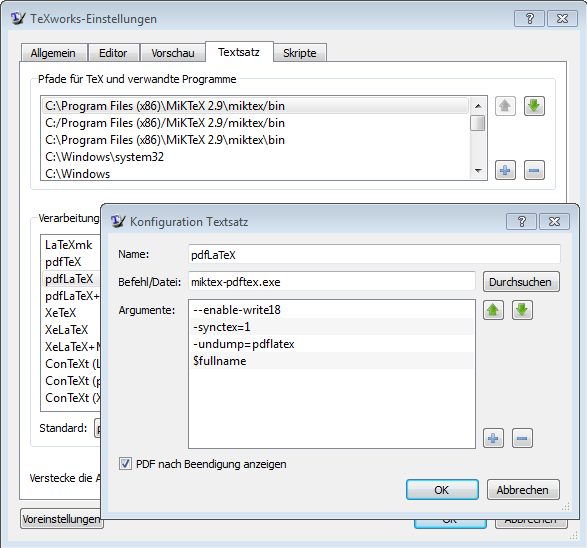
\includegraphics[width=0.9\textwidth]{img/pdfLatexSettingsForTexWorks.PNG}
   \caption{pdfLatex Settings in TexWorks}
   \label{img:pdfTexWorks}
\end{figure}

\begin{figure}[ht]
   \centering
   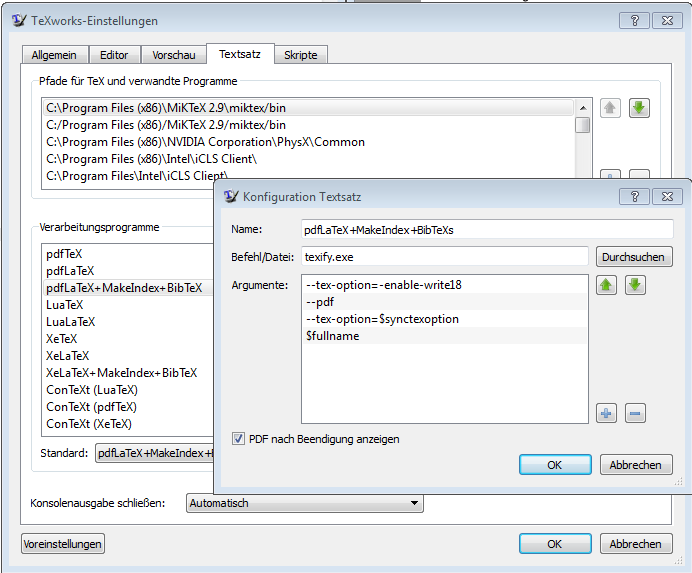
\includegraphics[width=0.9\textwidth]{img/pdfLatexMakeIndexBibTexSettingsForTexWorks.PNG}
   \caption{pdfLatex+MakeIndex+BibTex Settings in TexWorks}
   \label{img:pdfTexWorks2}
\end{figure}
\cleardoublepage
% !TeX root = /../Report.tex

\chapter{Working with \LaTeX\ }\label{sec:working}
This chapter explains how to typeset some of the most common elements contained in a technical report using \LaTeX.

\section{Headings}
Your report can be structured using several different types of headings. Use the commands \texttt{\textbackslash chapter\{.\}}, \texttt{\textbackslash section\{.\}}, \texttt{\textbackslash subsection\{.\}}, and \texttt{\textbackslash subsubsection\{.\}}. Use the asterisk symbol \texttt{*} to suppress numbering of a certain heading if necessary, for example, \texttt{\textbackslash section*\{.\}}.

\section{References and Footnotes}\label{sec:references}
References to literature are included using the command \texttt{\textbackslash
cite\{.\}}. For example \cite{optreg,motsys}. Your references must be entered in the file \texttt{bibliography.bib}. Making changes or adding new references in the bibliography file can be done manually or by using specialized software such as \textit{JabRef} which is free of charge.
 
Cross-referencing within the text is easily done using \texttt{\textbackslash label\{.\}} and \texttt{\textbackslash ref\{.\}}. For example, this paragraph is part of chapter~\ref{sec:working}; more specifically section~\ref{sec:references} on page~\pageref{sec:references}. You will need to compile your document twice in order for the cross-referencing to be updated.

Footnotes\footnote{The use of footnotes is generally not recommended.} are added using the command \texttt{\textbackslash footnote\{.\}}, but try to avoid the used of footnotes altogether.

\section{Lists}\label{sec:lists}
Three types of list-environments are commonly used: \texttt{itemize}, \texttt{enumerate}, and \texttt{description}. The following example uses \texttt{itemize} to create a list without numbering
\begin{itemize}
  \item point one; and
  \item point two
\end{itemize}
created using
\begin{verbatim}
\begin{itemize}
  \item point one; and
  \item point two
\end{itemize}
\end{verbatim}

The following example uses \texttt{enumerate} to create a list with numbering
\begin{enumerate}
  \item point one; and
  \item point two
\end{enumerate}
created using
\begin{verbatim}
\begin{enumerate}
  \item point one; and
  \item point two
\end{enumerate}
\end{verbatim}

The following example uses \texttt{description} to create a list with custom text as bullet-points
\begin{description}
  \item[P1] point one; and
  \item[P2] point two
\end{description}
created using
\begin{verbatim}
\begin{description}
  \item[P1] point one; and
  \item[P2] point two
\end{description}
\end{verbatim}


\section{Tables}\label{sec:tables}
Table~\ref{tab:table} shows an example of a simple table-layout. Try to avoid vertical lines on tables. The Internet contains countless resources on how to create special elements and structures in tables such as cells spanning multiple rows, rotated text, sideways tables, justification of cell elements, etc.
\begin{table}[h]
\begin{center}
\caption{Driving cycle data of ECE-15, EUDC, and NEDC.}\vspace{1ex}
\label{tab:table}
\begin{tabular}{llccc}\hline
Description & Unit & ECE & EUDC & NEDC \\ \hline
Duration & s & 780 & 400 & 1180 \\
Distance & km & 4.052 & 6.955 & 11.007 \\
Average velocity & km/h & 18.7 &  62.6 & 33.6 \\
Idle speed & \% & 36 & 10 & 27 \\ \hline
\end{tabular}
\end{center}
\end{table}

This table was created using
\begin{verbatim}
\begin{table}[h]
\begin{center}
\caption{Driving cycle data of ECE-15, EUDC, and NEDC.}\vspace{1ex}
\label{tab:table}
\begin{tabular}{llccc}\hline
Description & Unit & ECE & EUDC & NEDC \\ \hline
Duration & s & 780 & 400 & 1180 \\
Distance & km & 4.052 & 6.955 & 11.007 \\
Average velocity & km/h & 18.7 &  62.6 & 33.6 \\
Idle speed & \% & 36 & 10 & 27 \\ \hline
\end{tabular}
\end{center}
\end{table}
\end{verbatim}
Table~\ref{tab:table_advanced} shows a more advanced version of Tab.~\ref{tab:table} using the \texttt{booktabs} package. Inspect the source code of this document to see how this was done.
\begin{table}[h]
\begin{center}
\small
\caption{Driving cycle data of ECE-15, EUDC, and NEDC.}\vspace{1ex}
\label{tab:table_advanced}
\begin{tabular}{@{}lcccc@{}}\toprule[2pt]
& & \multicolumn{3}{c}{\bf Driving cycle}\\
\cmidrule{3-5}
Description & Unit & {ECE} & {EUDC} & {NEDC} \\ \midrule
Duration & \unit[]{s} & 780 & 400 & 1180 \\
Distance & \unit[]{km} & 4.052 & 6.955 & 11.007 \\
Average velocity & \unitfrac[]{km}{h} & 18.7 &  62.6 & 33.6 \\
Idle speed & \unit[]{\%} & 36 & 10 & 27 \\ \bottomrule[2pt]
\end{tabular}
\end{center}
\end{table}



\section{Working with Units}
The package \texttt{\textbackslash usepackage\{units\}} enables two useful commands, namely \texttt{\textbackslash unit[.]\{.\}} and \\ \texttt{\textbackslash unitfrac[.]\{.\}\{.\}}. Use these commands to display units in a concise way, for example
\begin{align}
\delta t &= \unit[1]{s}\\
v &= \unitfrac[5]{m}{s}.
\end{align}
This example was done using
\begin{verbatim}
\begin{align}
\delta t &= \unit[1]{s}\\
v &= \unitfrac[5]{m}{s}.
\end{align}
\end{verbatim}

\section{Including Graphics}\label{sec:epsgraph}
It is recommended that you only use encapsulated post-script graphics \texttt{.eps} in your report. If you mix \texttt{.eps} with other formats such as \texttt{.png}, \texttt{.jpeg} or \texttt{.gif}, you will most likely not be able to compile your report without errors. Note that figures created in \textsc{Matlab} are easily saved in \texttt{.eps} format.

The inclusion of a figure can be done in the following way:
\begin{verbatim}
\begin{figure}[ht]
   \centering
   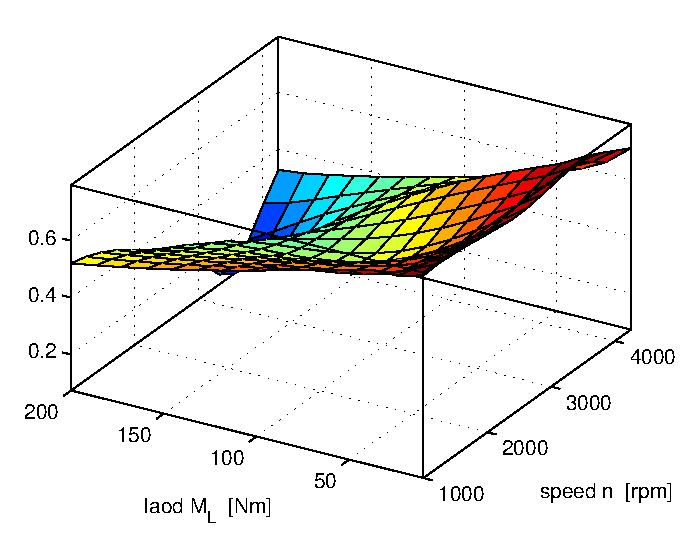
\includegraphics[width=0.75\textwidth]{img/k_surf.eps}
   \caption{Example of a figure.}
   \label{img:k_surf}
\end{figure}
\end{verbatim}

\begin{figure}[ht]
   \centering
   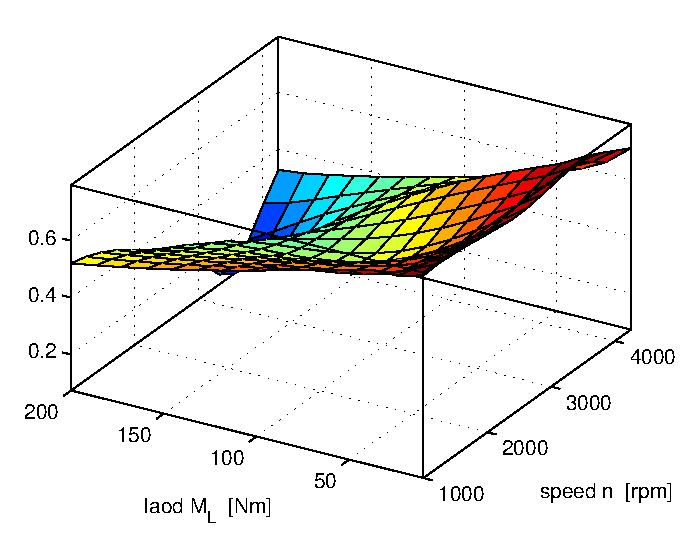
\includegraphics[width=0.75\textwidth]{img/k_surf.eps}
   \caption{Example of a figure.}
   \label{img:k_surf}
\end{figure}

Two figures are displayed next to each other using
\begin{verbatim}
\begin{figure}[h]
  \begin{minipage}[t]{0.48\textwidth}
    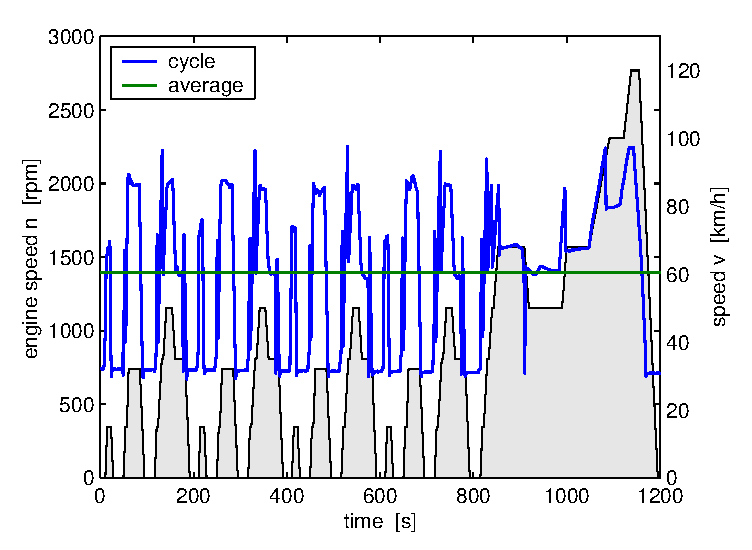
\includegraphics[width = \textwidth]{img/cycle_we.eps}
  \end{minipage}
  \hfill
  \begin{minipage}[t]{0.48\textwidth}
    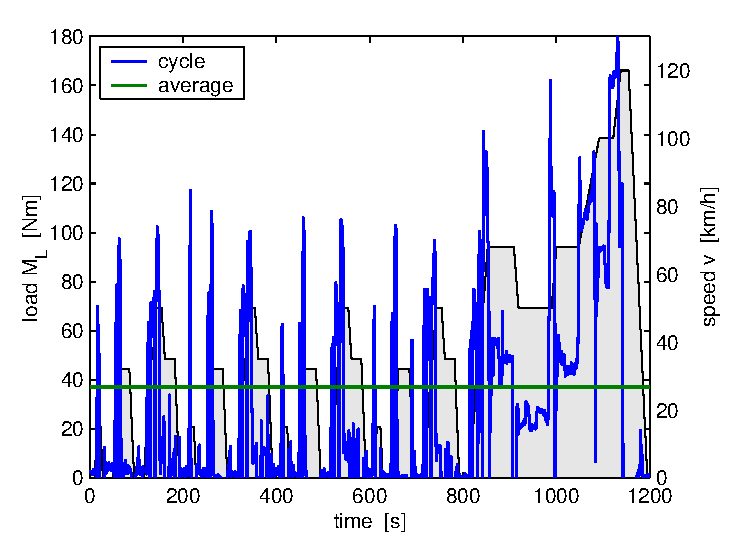
\includegraphics[width = \textwidth]{img/cycle_ml.eps}
  \end{minipage}
  \caption{Two figures next to each other.}
  \label{img:cycle}
\end{figure}
\end{verbatim}

\begin{figure}[ht]
  \begin{minipage}[t]{0.48\textwidth}
    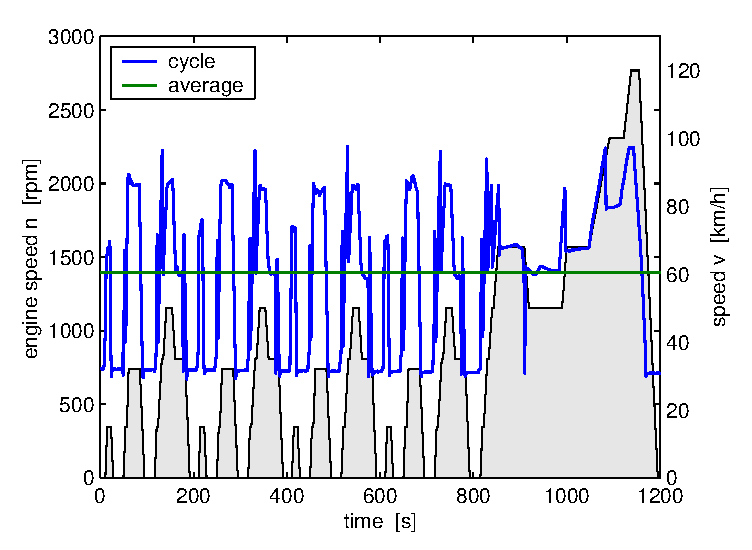
\includegraphics[width = \textwidth]{img/cycle_we.eps}
  \end{minipage}
  \hfill
  \begin{minipage}[t]{0.48\textwidth}
    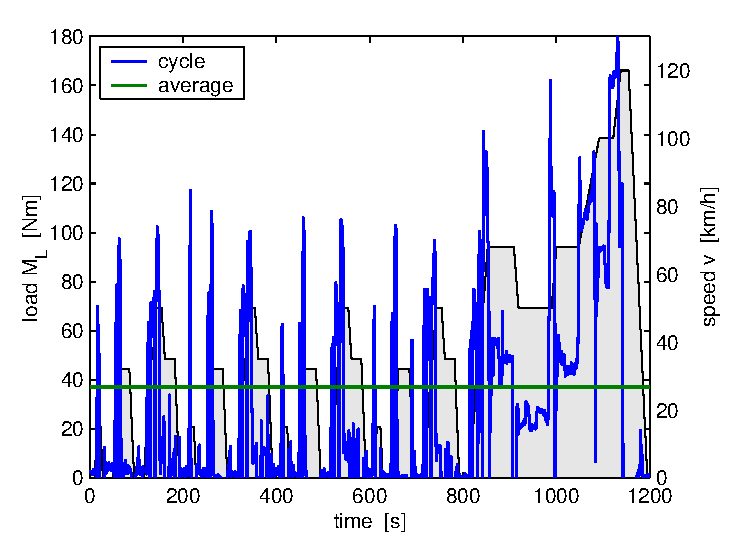
\includegraphics[width = \textwidth]{img/cycle_ml.eps}
  \end{minipage}
  \caption{Two figures next to each other.}
  \label{img:cycle}
\end{figure}

The positioning parameter \texttt{h} (here) forces your figure to be placed in the current position relative to your text. You may add \texttt{t} (top), \texttt{b} (bottom), and/or \texttt{p} (page) to allow for more flexible positioning within your document. For instance, \texttt{[tb]} forces your figure to be placed either on the top or bottom of a page.


\section{Equations}\label{sec:math}
The most common way to include equations is using the \texttt{equation} environment.
\begin{equation}\label{eq:p_me0f}
 p_\mathrm{me0f}(T_e,\omega_e) \ = \ k_1(T_e) \cdot (k_2+k_3 S^2
 \omega_e^2) \cdot \Pi_\mathrm{max} \cdot \sqrt{\frac{k_4}{B}} \, .
\end{equation}
It is recommended to use \texttt{\textbackslash mathrm\{.\}} for subscripts comprising more than two letters since it reduces the width of the subscript significantly and improves readability. The corresponding code is
\begin{verbatim}
\begin{equation}\label{eq:p_me0f}
 p_\mathrm{me0f}(T_e,\omega_e) \ = \ k_1(T_e) \cdot (k_2+k_3 S^2
 \omega_e^2) \cdot \Pi_\mathrm{max} \cdot \sqrt{\frac{k_4}{B}} \, .
\end{equation}
\end{verbatim}
Equations, such as Eq.~\eqref{eq:p_me0f}, may be referenced using \texttt{\textbackslash eqref\{.\}}. In-line mathematical content is created using \texttt{\$.\$}, for example $a^2+b^2=c^2$. It is practically possible to typeset any equation in \LaTeX. Equation~\eqref{eq:advanced} shows an example of a more advance structure.
\begin{equation}\label{eq:advanced}
x^k_n(i) = \left\{\begin{array}{ll}y(i) & \text{if}\quad x^k_{n-1}(i)\leq \mathbf{x}\\
z(i) & \text{otherwise}\end{array}\right., \text{for}\quad i=\{1,\ldots,N\}.
\end{equation}


\subsection{Vectors, Matrices and Derivations}

By means of easier understanding of equations, there are different standards how to imply a variable to be a scalar, vector or matrix.

We use the following:
\begin{itemize}
	\item scalar variables are normal math-mode characters, e.g. $m$
	\item Vector is a lowercase bold symbol e.g. $\V{v}$
	\item Matrix is an uppercase bold symbol e.g. $\M{A}$
\end{itemize}

If you want to speak about a variable in your text, make sure to enter math-mode. E.g. to write a variable for mass $m$ not to be confused with the unit m (for meter), use:
\begin{verbatim}
$m$
\end{verbatim}

Because vectors, matrices and a first derivative are often used we added to small commands for you to be used in math-mode:
$\V{v}$, $\M{A}$, $\D{x}{t}$, $\D{\V{v}}{t}$, where in the last two examples, $\D{x}{t}$ is a scalar time derivative and $\D{\V{v}}{t}$ a vector time derivative.
The code for these examples is: 
\begin{verbatim}
$\V{v}$, $\M{A}$, $\D{x}{t}$, $\D{\V{v}}{t}$
\end{verbatim}


\section{Including Code in your Document}
Include samples from your Matlab code using the \texttt{lstlistings} environment, for example
\lstset{language=Matlab,numbers=none}
\begin{lstlisting}[frame=lines]
% Evaluate y = 2x
for i = 1:length(x)

  y(i) = 2*x(i);

end
\end{lstlisting}
This example was created using
\begin{verbatim}
\lstset{language=Matlab,numbers=none}
\begin{lstlisting}[frame=lines]
% Evaluate y = 2x
for i = 1:length(x)

  y(i) = 2*x(i);

end
\end{lstlisting}
\end{verbatim}
where \texttt{\textbackslash usepackage\{mcode\}} must be included in the preamble of your document. If you want to include the entire content of a file \texttt{mycode.m} in your document, simply input the path to \texttt{mycode.m} instead of pasting the entire content into your \TeX -file
\begin{verbatim}
\lstset{language=Matlab,numbers=left}
\lstinputlisting{path/to/mycode.m}
\end{verbatim}
Including the path to your m-file also ensures that the code in your report is always up-to-date. The \texttt{\textbackslash lstset\{language=Matlab\}} command ensures that \textsc{Matlab} syntax definitions are used, but many other languages are recognised as well such as \texttt{Fortran} and \texttt{C++}.

\cleardoublepage
% !TeX root = /../Report.tex

\chapter{Scientific Writing}\label{scientificWriting}

This chapter contains some general hints for scientific writing.
Some of the hints and formulations are selected and copied sentences from \cite{zeiger2000ewb}, which can be found in the SMS library. Some of the other hints are stolen from a writing tutorial by Olivier, M-C and James from the ReLab\footnote{Rehabilitation Engineering Lab, ETH Zurich; www.relab.ethz.ch}.

\vspace{0.5cm}

Your goal when writing a scientific text should be clarity:
\begin{description}
	\item[Write clearly to ensure that your readers understand your message.] 
		``Clear writing is writing that is incapable of being misunderstood.'' Quintilian, \Cross ~96 A.D.  \hfill \\
		Readers have different scientific backgrounds, have different native languages and might be only half awake while reading your thesis. Clear writing helps to make them understand your message. \hfill \\
		Focus on short, meaty and clear formulations.
	\item[Write clearly to clarify your own thinking] Clear writing helps you to sort your thoughts. Clear writing does also help you to discover faulty reasoning (e.g. lapses in logic and inconsistencies).
\end{description}

\section{Word Choice}

Clarity starts with the choice of words.
For non native English writers this may be challenge in the beginning.
Feel free to use a dictionary (e.g. leo.org) that provides you with example sentences for given words.
It is often details in word choice that improve the reading. Most words that are carelessly taken as synonyms do not mean exactly the same, e.g. to increase versus to enhance:
\begin{description}
	\item[to increase] General term that means to become or to make greater in some respect, such as size, quantity, number, degree, value or intensity.
	\item[to enhance] Evaluative term that means to add to something that is already attractive, worthy of value, thus increasing its value.
\end{description}


\section{Abbreviations}

Abbreviations do generally have a bad influence on readability.
Therefore it is generally suggested to avoid using them with some exceptions:
\begin{itemize}
	\item Standard units of measurements (e.g. system international units)
	\item Widely accepted abbreviations, especially where you expect the readers to be more familiar with the abbreviation than with the whole word (e.g. DNA better than deoxyribonucleic acid, or LED rather than light emitting diode).
	\item When the full term is repeatedly used within the text and would clutter the paragraphs. However, the first time you use such an abbreviation within a section you should write the complete term and the abbreviation in brackets, e.g. ``Our novel generalized elastic path control (GEPC) allows to ...''.
Avoid multiple different abbreviations within sections, because it interrupts fluid reading.
\end{itemize}

Add the used abbreviations (except SI-units) to the symbols page at the beginning of this template in alphabetical order.

\section{Active Versus Passive}

Often people try to avoid ``We + active verb...'' sentences and use passive instead.
However, this does not necessarily improve the clarity of your message.
Try to use the passive tense only for standard procedures.
Whereas the ``We + active verb'' combination is to signal something that is new, unexpected or a personal choice out of many possibilities. 

\section{Sentence Structure}

\begin{description}
	\item[Express the core of the message in the subject, verb, and completer.]
		Make the topic the subject of the sentence.\hfill \\
		Put the action in the verb.\hfill \\
		E.g.: Use ``Heart rate increased." instead of "An increase in heart rate occurred.''.
	\item[Avoid noun clusters.] \hfill \\
		E.g.: Use ``variability of filament length'' instead of ``filament length variability''.
	\item[Write short sentences] \hfill \\
		Do not string ideas together. \hfill \\
		Talk about one thing at a time. \hfill \\
		Aim for a mean sentence length of no more than 22 words per sentence.
	\item[Use clear pronouns.] \hfill \\
		If there are to many nouns a pronoun could refer to, either restate the noun or change the sentence structure.\hfill \\
		For a pronoun (usually ``this'') that has no noun to refer to, add the smallest category term after the pronoun.	
	\item[Put parallel ideas in parallel form] \hfill \\
		Use parallel form for ideas joined by ``and'', ``or'', or ``but'' and for comparisons.	\hfill \\
		Use ``than'' for comparisons, not ``compared to''. \hfill \\ 
		Do not compare apples and oranges (E.g. correct sentences like ``Results are similar to previous studies.''). \hfill \\
		Do not write absolute statements in comparisons. \hfill \\
		Use parallel form to avoid repetition.
	\item[Avoid writing flaws.] \hfill \\
		Be sure that the subject and verb make sense together. \hfill \\
		Be sure the subject and the verb agree. \hfill \\
		Do not omit helping verbs. \hfill \\
		Be sure that sentences containing information in parenthesis make sense.
\end{description}

\section{Paragraph Structure}

To send a clear message and tell a clear story, paragraphs should be organized, should have continuity, and should emphasize important information.

Focus on:
\begin{description}
	\item[Organization of the paragraph] \hfill \\
		Give an overview in the first sentence (``topic sentence''). \hfill \\
		Then give details, in logically organized supporting sentences. \hfill \\
		Do not omit any steps on the logic. \hfill \\
		Try to sort the supporting sentences in the best fitting logic, e.g.  ``least to most important'', ``most to least important'', a previously announced order, ``pro-con'', ``chronological'', ``problem-solution'', ``solution-problem'' ... 
	\item[Continuity] \hfill \\
		Repeat key terms (exactly and early).\hfill \\
		Link key terms when you switch from a specific term to a category term, or vice versa.\hfill \\
		Use transition words, phrases, or clauses to indicate logical relationships between ideas.\hfill \\
		Keep a consistent order.\hfill \\
		Keep a consistent point of view if the topic of multiple sentences is the same.\hfill \\
		Use parallel form for parallel ideas. \hfill \\
		Signal subtopics within a paragraph.
	\item[Emphasis]
		It is your job to tell the reader what is important to you. \hfill \\
		Emphasize important information, place it in a power position, label it, repeat it, and state it rather than just implying it.  \hfill \\
		De-emphasize less important information, condense, omit, or place it or subordinate\footnote{to subordinate $\approx$ in einen Nebensatz umformulieren} it.
\end{description}

\section{About Citations and Plagiarism}\label{AboutPlagiarism}

There are different types of plagiarism. Some of them are obvious others might be unknown to you:
\begin{description}
	\item[The Ghostwriter] The author submits a paper in his/her name that in actual fact s/he commissioned another
person to write.
	\item[The Full Monty] The author submits the work of another author in his/her name.
	\item[Self-plagiarism] The author submits the same work (or extracts of the paper) for different seminars or exams.
	\item[Translation plagiarism] The author translates texts, or text extracts, from another language and submits them as his/her own work without citations.
\end{description}

Having incomplete or wrong citations can also lead to plagiarism.
\begin{description}
	\item[The Forgotten Citation] The author uses extracts of another author's work without citing that author. This also includes passages from the internet.
	\item[Paraphrase Plagiarism] The author paraphrases texts (i.e., changes them as deemed fit) from another author and does not quote them.
	\item[Poorly located citation] The author uses extracts of another author's work, perhaps paraphrasing them, and cites the work, but not in the context of the passages used.
	\item[The Forgotten Footnote] The writer mentions an author's name for a source, but neglects to include specific information on the location of the material referenced. This often masks other forms of plagiarism by \textbf{obscuring source locations}.
	\item[The Misinformer] The \textbf{writer provides inaccurate information regarding the sources}, making it impossible to find them.
\end{description}

The devil is sometimes in the detail, paraphrasing wrongly can also be declared plagiarism:
\begin{description}
	\item[The Too-Perfect Paraphrase] The writer properly cites a source, but \textbf{neglects to put in quotation marks} text that has been copied word-for-word, or close to it. Although attributing the basic ideas to the source, the writer is falsely claiming original presentation and interpretation of the information.
	\item[The Resourceful Citer] The writer properly cites all sources, paraphrasing and using quotations appropriately. The catch? \textbf{The paper contains almost no original work!} It is sometimes difficult to spot this form of plagiarism because it looks like any other well-researched document.
	\item[The Perfect Crime] Well, we all know it doesn't exist. In this case, the writer properly quotes and cites sources in some places, but goes on to paraphrase other arguments from those sources without citation. This way, the \textbf{writer tries to pass off the paraphrased material as his or her own analysis of the cited material}.
\end{description}

If you do have questions how to cite or paraphrase a source correctly, point it out and discuss it with your supervisor.
He will be able to help you, provides some examples or suggests alternatives.



\section{Structure of Your Thesis}

For different scientific topics or research fields, different structures may be optimal.
A classical structure for a hypothesis based thesis would be:
\begin{enumerate}
	\item Abstract
	\item Introduction
	\item Material and Methods
	\item Results
	\item Discussion and Conclusion
	\item References/Bibliography
\end{enumerate} 
However, for a technical thesis this might not be optimal and therefore adaptations to this structures may be beneficial.

With this template you are already given a general structure for your report consisting of:
\begin{enumerate}
	\item Title page
	\item Abstract and ``\"Uebersicht''
	\item Acknowledgments
	\item Declaration of Originality
	\item Symbols
	\item Introduction
	\item \textasteriskcentered Related Work\textasteriskcentered
	\item \textasteriskcentered Own Work\textasteriskcentered
	\item Results and Discussion
	\item Conclusion
	\item Appendix
	\item Bibliography
\end{enumerate} 

The \textasteriskcentered Related Work\textasteriskcentered ~and  \textasteriskcentered Own Work\textasteriskcentered ~are placeholders to be replace with your actual chapters.
They are the analogue to the classical "Material and Methods" from a hypothesis based thesis.

The \textasteriskcentered Related Work\textasteriskcentered ~ chapter can usually be replaced with one or multiple chapters that provide necessary knowledge to the reader to understand the Materials you are working with.
The \textasteriskcentered Own Work\textasteriskcentered  ~ chapter can then be replaced by your own Material and Methods part, where describe what you actually have developed or tested.

These two chapters stand for the part of the thesis structure, where you are supposed to adapt the this template to your needs.
You will find more information and examples in the respective ``dummy'' chapters of this template.

This structure is not set in stone. 
You can always ask your supervisor for additional changes.

%------------------------------------------------------------------------------------------------------------------------
\section{Abstract}\label{AboutAbstract}

What is an Abstract?
\begin{itemize}
	\item Brief, accurate, and comprehensive summary of the contents of the article without added interpretation or criticism.
	\item Quick idea of the paper.
	\item Short sentences, each covering one specific topic.
	\item Present the quantitative and/or qualitative information contained in the document.
	\item Does not contain subsections, figures and tables.
	\item The \textbf{only} part of you work that will be read by 90\% of the people that offered to read your thesis.
\end{itemize}

An abstract should be clearly structured and contain the following components in the given order:
\begin{description}
	\item[Background information] What is known of the problem? Use Present or present perfect (describe facts).
	\item[Purpose of the study] Why did I do this? Use Past (or present) tense.
	\item[Methods]  What did I do? Use Past tense.
	\item[Results (major)] What did I find? Use Past (or present) tense.
	\item[Conclusions/implications] What does it mean? Use Present/conditional tense.
\end{description}

Usually it is recommended to write the abstract at the end.
Personally, I recommend you to write an incomplete first draft as early as possible and try to keep it up to date with your progress.
Even if you will completely rewrite the abstract in the end, the process of updating, editing and changing this compact summery of your thesis may help you to keep focus on the important aspects of your work.

%------------------------------------------------------------------------------------------------------------------------
\section{Introduction}\label{AboutIntroduction}

Aim: create a research space or a niche for the research.

\begin{description}
	\item[Move 1 Establishing a research territory] \hfill \\
	\begin{enumerate} 
		\item by showing that the general research area is important, central, interesting, problematic, or relevant in some way.
		\item by introducing and reviewing items of previous research in the area.
	\end{enumerate}
	\item[Move 2 Establishing a niche] \hfill \\
		\begin{itemize}
			\item by indicating a gap in the previous research, raising a question about it, or
			\item showing the need to extend previous knowledge in some way.
		\end{itemize}
	\item[Move 3 Occupying the niche] \hfill \\
	\begin{enumerate}
		\item by outlining purposes or stating the nature of the present research
		\item by announcing principal findings
		\item by indicating the structure of the article
	\end{enumerate}
\end{description}

N.B. Many introductions consist of more that one sequence of moves 1 \& 2, as there are different strands of the research background that lead to different kinds of gaps in the research record. 

\subsection{Move 1: Tense choice when citing the literature}\label{tenseChoice}
	
	\begin{description}	
		\item[Present (reference to state of current knowledge)] \hfill \\
		\begin{itemize}
			\item ``Stroke \textbf{is} the leading cause of permanent disability in the United States $[$1$]$.''
			\item ``The prognosis of untreated patients \textbf{is} poor... $[$1,~2$]$''
		\end{itemize}
		\item[Past (reference to single studies)] \hfill \\
		\begin{itemize}
			\item ``Twenty-five years ago, the prevailing view \textbf{held} that axons project randomly, and that only productive interactions \textbf{were stabilized} and would persist (Pettigrew et al., 1979).''
			\item ``Farah, Peronnet, Gonon and Girard (1988) \textbf{used} evoked potentials to study visual imagery, and \textbf{found} activity on the posterior scalp ...''
		\end{itemize}
		\item[Present Perfect (reference to areas of inquiry)] \hfill \\ 
		\begin{itemize}
			\item ``At present, an increasing number of studies \textbf{have shown} beneficial effects of exercise training in MS... $[$1,~2$]$''
			\item ``Metrics extracted from movement data recorded from patients undergoing MIT- Manus therapy \textbf{have been used} for quantifying patients motor abilities and their changes during motor recovery and \textbf{have offered} unprecedented insights into the process of motor recovery from stroke $[$16-18$]$.''
		\end{itemize}
	\end{description}

\subsection{Move 2: Establishing a niche}

In many ways, \textbf{move 2 is the key move} in introductions. It is the hinge that connects move 1 (what has been done) to move 3 (what the present research is about). Move 2 thus establishes the \textbf{motivation} for the study.

Most move 2s establish a niche by \textbf{indicating a gap} - by showing that the research story so far is incomplete. Sometimes they take the form of a critique. They are usually quite short, often consisting of no more than a sentence.

Examples:
\begin{itemize}
	\item ``\textbf{However}, the previously mentioned methods suffer from some limitations...''
	\item ``\textbf{Unfortunately}, the outcomes of exercise therapy on arm function in MS have hardly been investigated.''
	\item ``\textbf{It remains unclear} how these robot-based kinematic and kinetic metrics relate to traditional human- administered clinical scales for measuring outcome.''
\end{itemize}

\subsection{Move 3 - Occupying the niche}

The third and final step in the typical research paper introduction is to make an offer to \textbf{fill the gap} (or answer the question) that has been created in move 2. The first part of move 3 (stating the nature of the present research) is obligatory.

Examples of beginning of move 3:
\begin{enumerate}
	\item ``The main objectives of the present paper are ...''
	\item ``This paper reports on results obtained ...''
	\item ``Here we give preliminary results for ...''
	\item ``The main purpose of the experiment reported here was to ...''
	\item ``This study was designed to explore ...''
	\item ``The present work extends previous ...''
	\item ``We now report on several ...''
	\item ``The primary focus of this paper is on ...''
	\item ``The aim of this investigation was to test ...''
	\item ``In this paper we show for the first time ...''
\end{enumerate}

%------------------------------------------------------------------------------------------------------------------------
\section{Related work}\label{relatedwork}

The idea of splitting Materials and Methods into at least two different chapters is based on the idea that you find a clear separation between your own and already existing work in your field.
This is generally just a recommendation and you do not need to stick with these chapters as such.

The ``Related Work'' chapter can be replaced by a chapter ``Theory'' for example, where you provide a summary of definitions or describing the theoretical knowledge, which you did not discover, but is needed to understand your work.
Another example chapter for ``Related Work'' could be introducing materials (e.g. a robot, other hardware or development environment) to the reader, which you use, but did not design/develop.
If you have an extensive literature research, which does not fit into the introduction, this is also the place to introduce a chapter about the state of the art or preliminary research.

Remember to use the present for facts or the state of current knowledge (e.g. in theoretical parts) and past for references as explained in section~\ref{tenseChoice}.

It is sometimes easier to start describing your own work in chapter~\ref{ownwork} and then figure out, what theory or background you have to introduce to the reader here.

%------------------------------------------------------------------------------------------------------------------------
\section{Own work}\label{ownwork} 

The own work chapter is the place, where you actually document your own work, such as your methods, design procedures and development steps.
It is most related to a classical Material and Methods part.
Feel free to change the chapter topic or split your work into multiple chapters (e.g. Simulations and Experiments on the Robot or Implementation and Testing).

The following List shows what a classical Method chapter usually contains:

\begin{itemize}
	\item study design, e.g. different groups
	\item materials, e.g. robotic device, experimental setup, etc.
	\item subjects, e.g. type, age, number, etc
	\item experimental procedures
	\item measurement methods, e.g. how are specific signals recorded
	\item calculations/data analysis, e.g. how are the data treated, filtered, etc.
	\item statistical analysis, e.g. type of statistical tests, level of significance, etc.
\end{itemize}

You may have covered some of these points already in a ``Related Work'' chapter.
Do not introduce them redundantly.
However, it is often suited to remind the reader with a reference to previously explained content.
E.g.: ``The subject's rowing skills were assessed with the M$^3$ rowing simulator (introduced in section 3.2).''

\section{Results}\label{AboutResults}

For technical papers it may be challenging to separate results and discussion into their own sections, but try as good as you can not to mix results and interpretations.

Feel free to split Results and Discussion into two separate chapters instead of only having two separate sections.

The \textbf{Results section is the core of the thesis} to which everything else relates, and should therefore be written first (or after you have written the methods). 	

The aim is to \textbf{present and illustrate your findings}. Make this section a \textbf{completely objective} report of the results, and \textbf{save all interpretation for the discussion}.

For engineering works or technical implementations it is sometimes challenging to create an interesting results section.
However, try to report as objective as possible, if the introduced design goals or criteria from the ``Methods'' section are met.

Structure of results section:
\begin{enumerate}
	\item Main result
	\item Supporting details (change, significance)
	\item Secondary result
	\item Supporting details (change, significance)
\end{enumerate}

Guidelines for writing the results:
\begin{description}
	\item[Report the results as clearly and concisely as possible.] \hfill \\
		 	Keep data to a minimum in the text (use figures and tables).
	\item[Give a clear idea of the magnitude of a response or difference.]
		Report percent changes or differences rather than quoting exact data.
	\item[Organize results.] Report them either chronologically, from most to least important or in a previously introduced sorting (e.g. same order as evaluation criteria introduced in methods). Point the reader to observations that are most relevant.
	\item[Streamline results by] \hfill \\
		condensing them to avoid repetition; do not present your data more than once.\hfill \\
		not starting paragraphs with figure legends and titles, but by putting these in brackets.\hfill \\
		presenting data after stating the result they support.
	\item[Use the figure legends or table footnotes] to describe the experiment. If this is done, do not describe the experiment again in the text. \textbf{The text and legends should complement}, not overlap, each other.
	\item[Use past tense when you refer to your results.]
\end{description}

\section{Discussion}\label{AboutDiscussion}

The aim is to \textbf{provide an interpretation of your results and a support for all of your conclusions}, using evidence from your experiment and generally accepted knowledge.

 \textbf{Do not be superficial or restate the results or introduction - why did you find these results, what does it mean??}

Elements of a discussion:
\begin{itemize}
	\item If your results differ from your hypothesis, explain why that may have happened. If your results agree, then describe the theory that the evidence supported.
	\item You must relate your work to the findings of other studies, including previous studies you may have done and those of other investigators.
	\item \textbf{Consider alternative explanations of the findings.} It is easy to consider only those explanations that fit your bias.
	\item Draw conclusions based upon the results that you have and explain our new understanding of the problem you investigated.
	\item You may suggest future directions, such as how the experiment might be modified to accomplish another objective.
\end{itemize}

What to avoid in a discussion:
\begin{itemize}
	\item Overpresentation of the results (these should be in the result section).
	\item Do not introduce new results in the Discussion.
	\item The significance of findings should be clearly described, but avoid inflation of the importance of the findings.
	\item Unjustified speculation.
	\item Conclusions that are not supported by the data.
\end{itemize}

\section{Summary} \label{AboutSummary}

This is a general summary covering your complete thesis from introduction to discussion.
It is basically an extended abstract that does give closer overview about your methods used and also contains the most important results of your work.

Do not put any new information in the summary that has no original space within your thesis.

\section{Conclusion} \label{AboutConclusion}

The conclusion is basically your summary of the results and discussion.
Describe your impact, limitations and findings.

However, do not introduce new findings or ideas within the conclusion.
New stuff is in the discussion, here only the core findings of your discussion are emphasized.

\section{Future work} \label{AboutFuturework}

Based on your results, discussion and conclusions here you can give hints, possible new research questions or just a description how the project is proceeding.

Avoid general phrases.

State, specific on your results and findings:
\begin{itemize}
	\item where open questions remain.
	\item in what direction more work is required to reach your goal.
	\item what questions can now be addressed based on your work.
\end{itemize}

\cleardoublepage
% ...
% \input{}
% \cleardoublepage
% \input{}b
% \cleardoublepage
% ...
% !TeX root = /../Report.tex

\chapter{Results and Discussion}\label{resultsDiscussion}


\section{Results}\label{results}



\section{Discussion}\label{discussion}
\cleardoublepage
% !TeX root = /../Report.tex

\chapter{Conclusion}\label{chap:conclusion}


\section{Summary} \label{summary}


\section{Conclusion} \label{conclusion}


\section{Future work} \label{futurework}

\cleardoublepage

% Appendix______________________________________________________________________
\appendix
% !TeX root = /../Report.tex

\chapter{Something}\label{sec:something}

Put things for completeness here, to which you refer, but which are not part of the grading.
E.g. Reference tables, source code examples \dots

 \cleardoublepage


\chapter{Again Something}\label{sec:again_something}

Blah, blah \dots

 \cleardoublepage



% Bibliography__________________________________________________________________
% Literature (Additional references can be added to the .bib-file manually, or by using, for example, the free application JabRef). Compile in the following order: latex -bibtex -latex -latex

%Bibliographie
%bibliography
\bibliographystyle{plain}
\bibliography{bibliography}
\cleardoublepage

\end{document}